\documentclass[10pt]{article}
\textheight=9.25in \textwidth=7in \topmargin=-.75in
 \oddsidemargin=-0.25in
\evensidemargin=-0.25in
\usepackage{url}  % The bib file uses this
\usepackage{graphicx, wrapfig, lipsum} %to import pictures
\usepackage{amsmath, amssymb}
\usepackage{theorem, multicol, color}
\usepackage{gfsartemisia-euler}

\setlength{\intextsep}{5mm} \setlength{\textfloatsep}{5mm}
\setlength{\floatsep}{5mm}
\setlength{\parindent}{0em} % new paragraphs are not indented
\setcounter{MaxMatrixCols}{20}
\usepackage{caption}
\captionsetup[figure]{font=small}


%%%%  SHORTCUT COMMANDS  %%%%
\newcommand{\ds}{\displaystyle}
\newcommand{\Z}{\mathbb{Z}}
\newcommand{\arc}{\rightarrow}
\newcommand{\R}{\mathbb{R}}
\newcommand{\N}{\mathbb{N}}
\newcommand{\Q}{\mathbb{Q}}
\renewcommand{\P}{\mathbb{P}}
\newcommand{\blank}{\underline{\hspace{0.33in}}}
\newcommand{\qand}{\quad and \quad}
\renewcommand{\stirling}[2]{\genfrac{\{}{\}}{0pt}{}{#1}{#2}}
\newcommand{\dydx}{\ds \frac{d y}{d x}}
\newcommand{\ddx}{\ds \frac{d}{d x}}
\newcommand{\dvdx}{\ds \frac{d v}{d x}} 
\newcommand{\solution}{\color{blue} Solution: \color{black}}
%%%%  footnote style %%%%

\renewcommand{\thefootnote}{\fnsymbol{footnote}}

\pagestyle{empty}

\begin{document}

\begin{flushright}
Chandler Justice - A02313187
\end{flushright}
\noindent \underline{\hspace{3in}}\\
\textbf{MATH6400:} Quiz \#7\\
\textbf{Due:} April 4, 2026 @ 23:59\\

	
	\begin{enumerate}
		
		\item Make the supposed proof given by spaghettifying the circle rigorous using Eudoxus's Method of Exhaustion.  
		Please include in your proof an argument showing that the shape made with the spaghetti from the circle is in fact a triangle.\\

        \solution\\
        \textbf{Claim:} the area of the circle is $1/2 C r$, where $C :=$ circumference of the circle and $r := $ radius of the circle.\\

        \textbf{Proof:} Let $\pi := C/D = C/2r$, where $C :=$ circumference of the circle, $D :=$ diameter of the circle, and $r :=$ the radius of the circle. As shown in the figure in the original homework, start by dividing the circle into $n$ annuli and then ``flatten'' each annuli into a rectangle\footnote{In class, you talked about how this being allowed is questionable, but to me it makes sense because the flattened annuli and the original sliced annuli are topologically identical. I also got a C+ in the intro to topology class so my confidence in anything topology is weak at best}, we will call these flattened annuli ``strips''. Lets proceed by describing the strips.\\

        Each strip will have a unique length depending on where in the circle it originated from. The outermost (now \textit{strippified}) annulus will have length $C$ and the height will be $r/n$, where $n :=$ number of annulus. All annulus will have uniform height $r/n$ by construction. The next annulus will then have length $C - C/n$. The inner most annulus will have length $C - ((n-1)C)/n) = C/n$. We can see the difference in length between any subsequent strips is always $C/n$. Since these strips are decreasing uniformly in length, they can be arranged in a ragged triangle. We can then fit these strips into a triangle with height $r$ and length $C$ which has area $1/2Cr$ as shown in the figure below.

        \begin{center}
            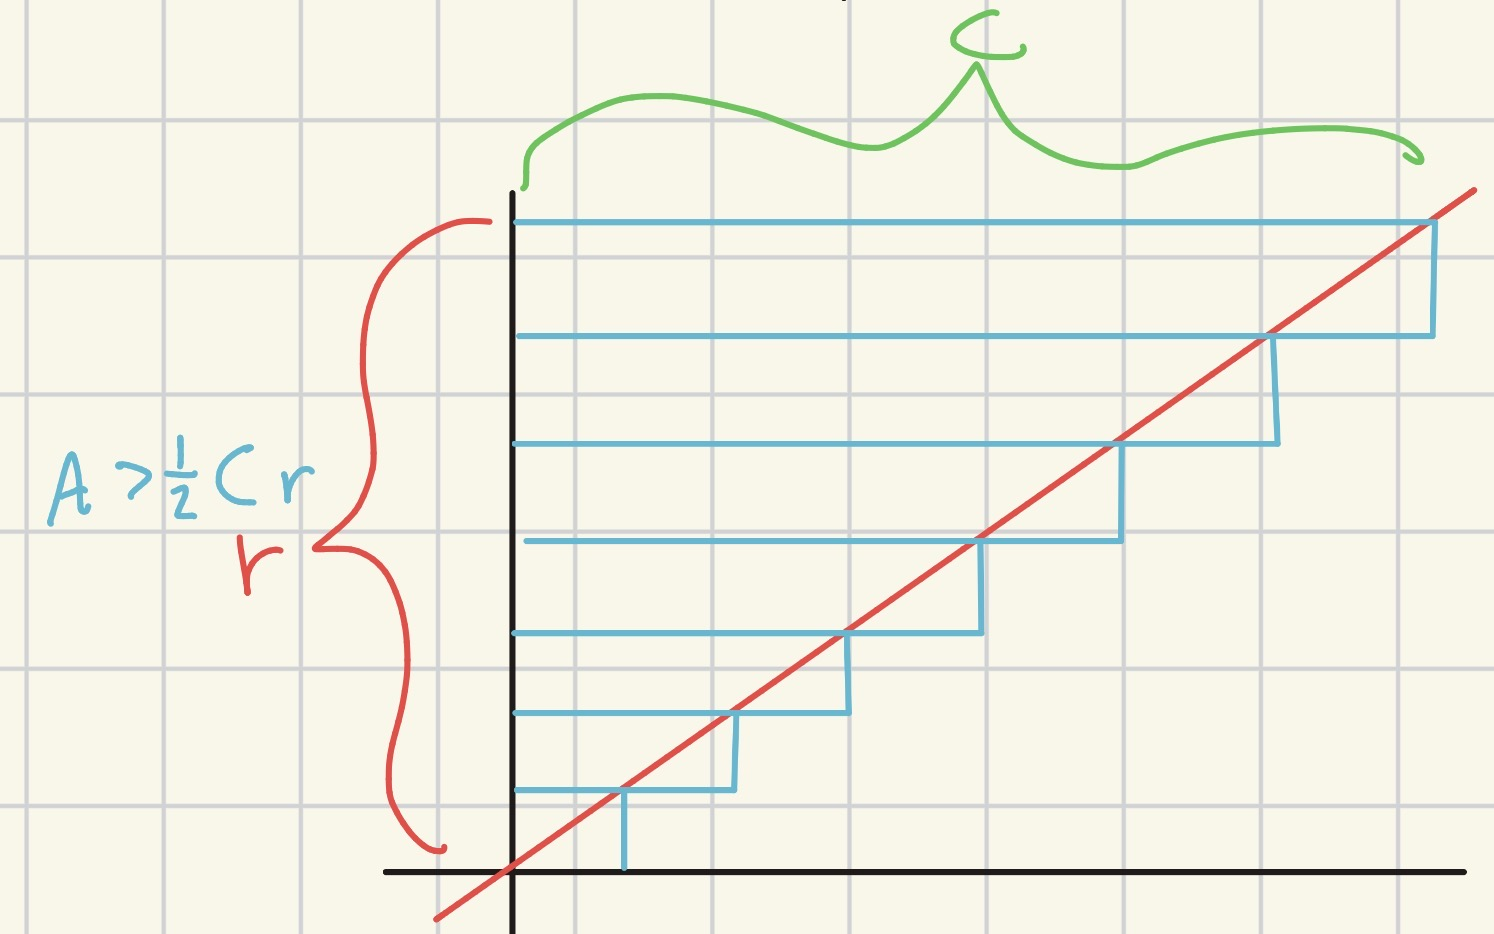
\includegraphics[scale=0.18]{over-estimate.jpg}
        \end{center}
        
        We can see this is an over-estimate of the triangle, and therefore the area represented by the strips is $> 1/2 Cr$. The area described by this arrangement is
        \[a(\text{arrangement}_1) = \sum_{i=1}^n 2C\pi \frac{i}{n} \frac{r}{n}\]
        We can see $2C \pi (i/n)$ is the length of each strip and $r/n$ is the width. Observe we can then create an under estimate by adjusting the bounds of the summation as shown in the figure below.
        \begin{center}
            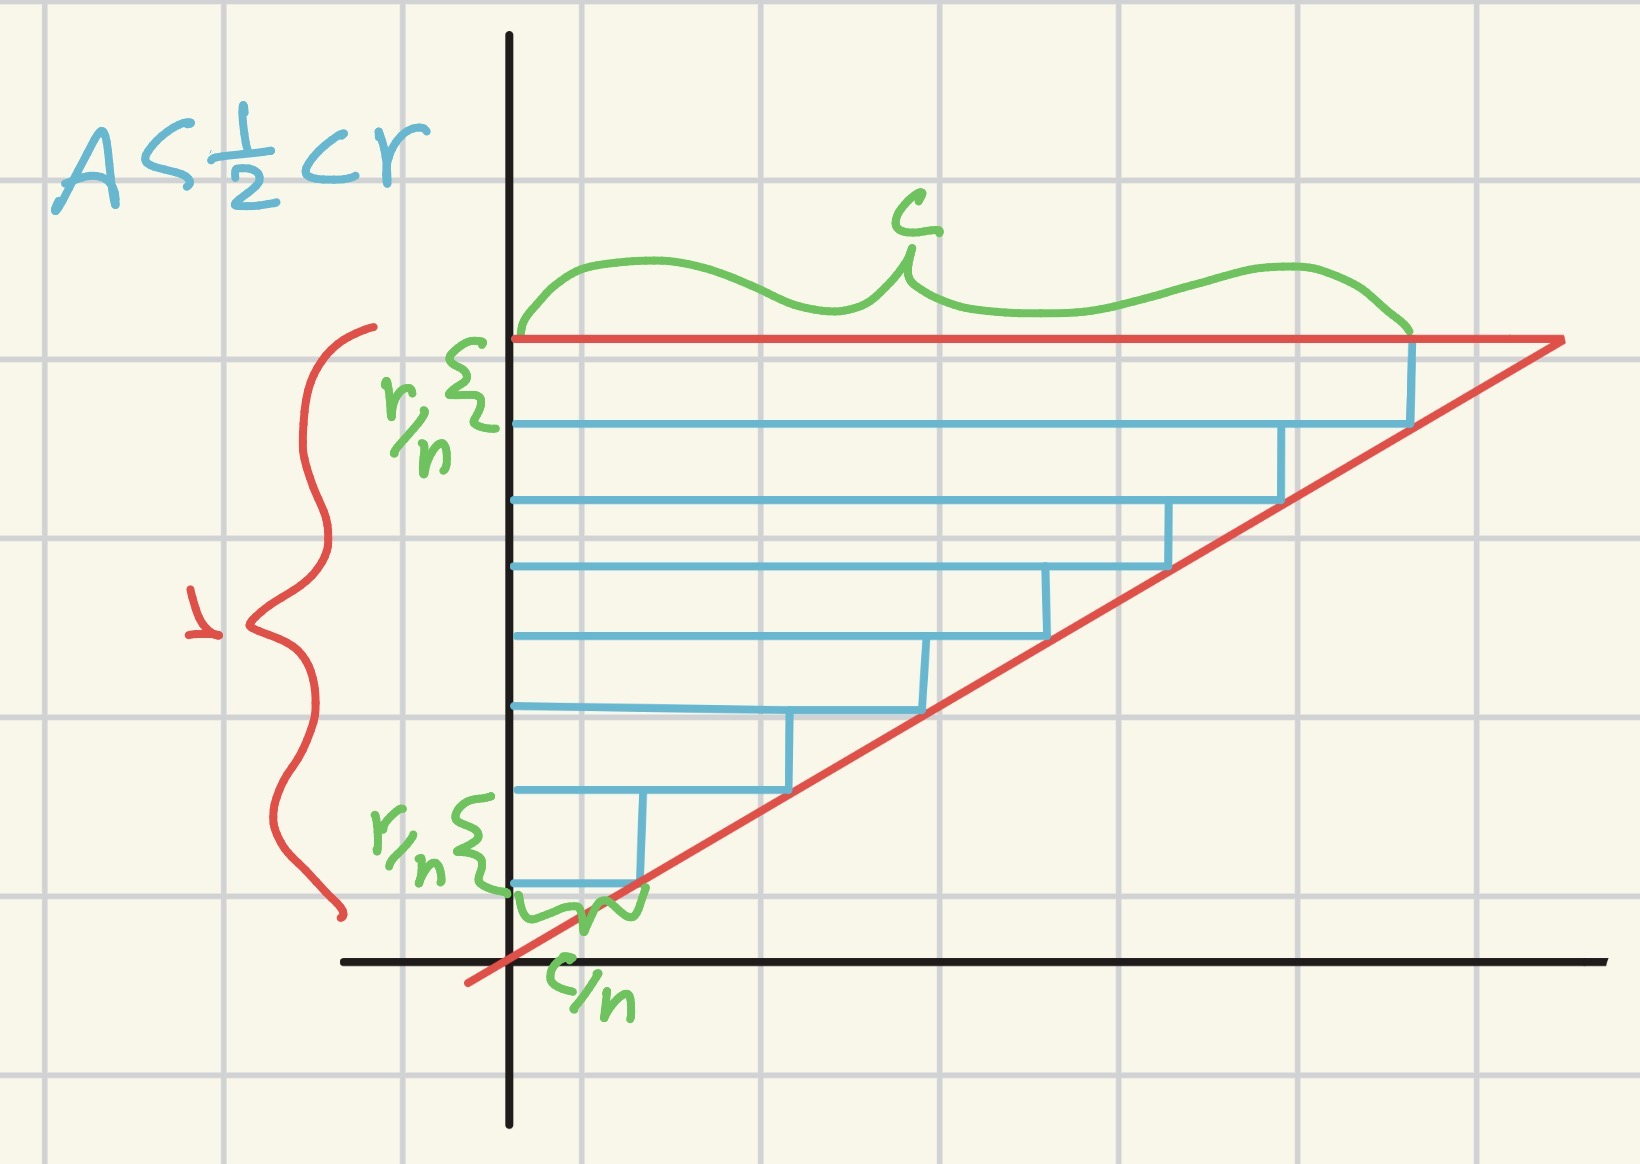
\includegraphics[scale=0.15]{under-estimate.jpg}
        \end{center}

        The area of these strips is then
        \[a(\text{arrangement}_2) = \sum_{i=0}^{n-1} 2C\pi \frac{i}{n} \frac{r}{n}\]

        From these summations and the triangle we are approximating, we can then see the following inequality
        \[\sum_{i=0}^{n-1} 2C\pi \frac{i}{n} \frac{r}{n} < \frac{1}{2} Cr < \sum_{i=1}^{n} 2C\pi \frac{i}{n} \frac{r}{n}\]

        \begin{center}
            
\includegraphics[scale=0.2]{meme.png}
        \end{center}
        
        Observe for any $\epsilon > 0$, there exists $n \gg 1$ such that
        \begin{align*}
            \sum_{i=0}^{n-1} 2C\pi \frac{i}{n} \frac{r}{n} - \frac{1}{2} Cr &< \epsilon\\
            \sum_{i=1}^{n} 2C\pi \frac{i}{n} \frac{r}{n} - \frac{1}{2} Cr &< \epsilon
        \end{align*}

        Therefore, we can see our under- and over- approximations of the triangle approach $1/2Cr$ for $n \gg 1$. Since the strips were originally constructing a circle, we can then see that as the error diminishes the ragged triangle created by the strips also approximates the area of the circle. Therefore, $a(\mathbb{C}) = 1/2Cr$. $\hfill\blacksquare$

		\item Let $a(\cdot)$ denote the area function.  Let $C_r$ denote a (the) circle with radius $r$. Prove that $a(C_r) = \pi r^2$ using the following:
		\begin{itemize}
			\item Define the area of a (the) circle with radius equal to $1$ to be $\pi$.
			\item Euclid's Proposition 2 from Book XII.
		\end{itemize}
		
		\item \noindent In class on 4/1 I presented the method Newton used to determine the coefficients $a_i$ in what-we-now-call the power series expansion of $(1+x)^{1/2}$. Newton discovered 
		$$(1+x)^{1/2} = 1 + \frac{1}{2}x - \frac{1}{8}x^2 + \frac{1}{16}x^3 -\frac{5}{128}x^4 + \frac{7}{256}x^5 - \cdots.$$
		More generally, using the notation $\alpha^{\underline{k}} = \alpha(\alpha -1)(\alpha -2)\cdots (\alpha - k + 1)$, where $k$ is a nonnegative integer, Newton discovered 
		\begin{eqnarray}(1+x)^{1/2} = 1 + \frac{1}{2}x + \frac{(1/2)(1/2-1)}{2}x^3 + \frac{(1/2)(1/2-1)(1/2-2)}{6}x^3 + \cdots + \frac{(1/2)^{\underline{k}}}{k!}x^k+ \cdots. \label{NewtonSeries}
		\end{eqnarray}
		
		
		
		\begin{enumerate}
			
			\item Use the fact $$\frac{\pi}{4} = \int_0^1 (1-x^2)^{1/2}dx$$
			together with (\ref{NewtonSeries}) to approximate $\pi$.  
			That is, expand the integrand as a power series and then integrate (some finite portion of) it term-by-term to obtain the approximation.  Experiment with accuracy, taking for granted that 
			$\pi \approx 3.1415926535$.  
			Newton knew Vi\'{e}te's approximation for $\pi$ obtained via a regular $6\cdot 2^{16}$-gon, and used that approximation to verify correctness of his method.  How many terms does Newton's result require to obtain $5$ digits of accuracy? 
			
			\item Showing insight into what-we-now-call ``\emph{convergence}'', Newton used a clever relationship to calculate $\pi$ with more accuracy than the integral in the above prompt affords. Newton used the fact that  
			\begin{eqnarray}\frac{\pi}{24} - \frac{\sqrt{3}}{32} = \int_0^{1/4} \sqrt{x-x^2}dx = \int_0^{1/4} x^{1/2}(1-x)^{1/2}\,dx.\label{NewtonArea}\end{eqnarray}
			Use (\ref{NewtonArea}) together with (\ref{NewtonSeries}) to approximate $\pi$.  
			Note that (\ref{NewtonArea}) yields 
			$$ \pi = 24\left(\int_0^{1/4}x^{1/2}(1-x)^{1/2}dx \right) + \frac{3}{4}\sqrt{3},$$
			and $\sqrt{3} = 2\sqrt{3/4} = 2\left(1-\frac{1}{4}\right)^{1/2}$.
			Please experiment with, and comment on, the accuracy of this approach, again taking for granted that $\pi \approx 3.1415926535$.
			
			
		\end{enumerate}
	\end{enumerate}


\noindent \underline{\hspace{3in}}\\

\end{document}

